\subsection{Hyperball-line picking}
\label{sec:hyperball_line}

The $n$-Dimensional hyperball is ...

Figure~\ref{fig:hyperball_eg} shows a 2D example (i.e., the
``disk''-line picking problem).

\begin{figure}[tbp]
  \begin{center}
    \subfloat[\label{fig:hyperball_eg}2D Hyperball
    Example.]{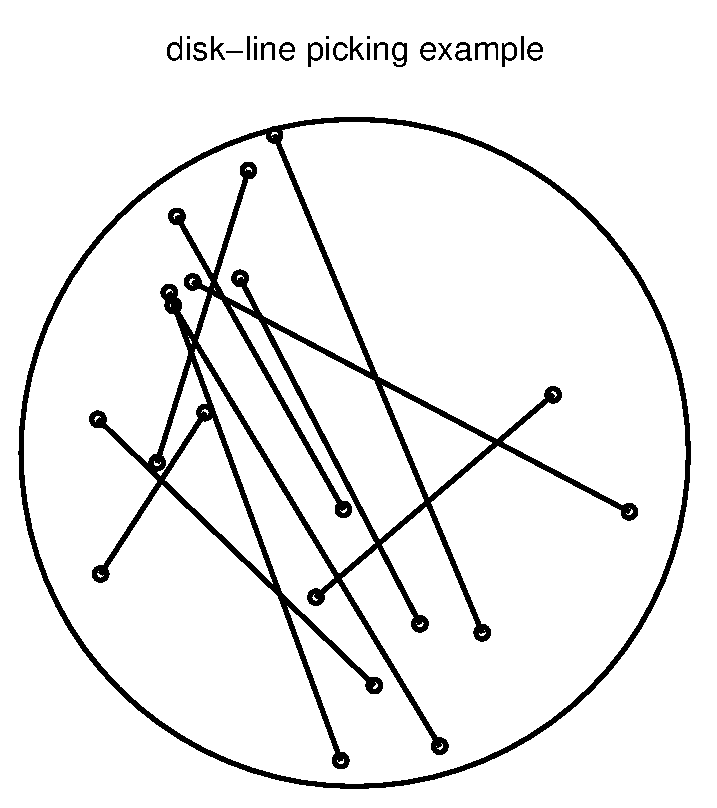
\includegraphics[width=0.4\columnwidth]{../Matlab/Plots/LinePicking_test_sim_disk_eg.eps}} 
    \hspace{6mm}
    \subfloat[\label{fig:hyperball_pdf}PDF of $n$-D Hyperballs.]{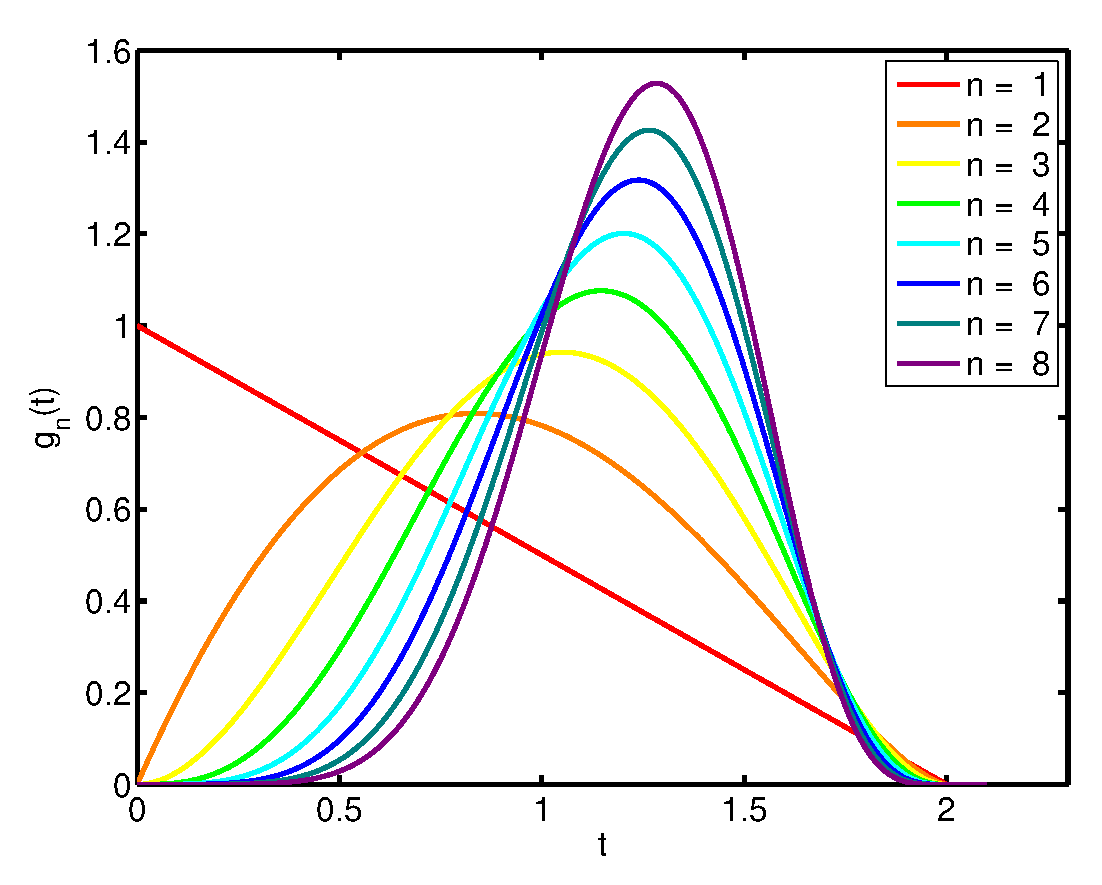
\includegraphics[width=0.48\columnwidth]{../Matlab/Plots/LinePicking_test_balls.eps}}
    \caption{The hyperball-line picking problem.}
  \end{center} 
\vspace{-4mm}
\end{figure}

\subsubsection{PDF}

Another obvious region on which to solve the line-picking problem is
the ball in $n$-dimensions~\cite{tu00:_circle_line} (equations
(27-31)). For a $n$-dimensional ball of radius $R$,
\begin{equation}
 g^{nD-{\rm ball}}_R(t) = n \frac{t^{n-1}}{R^n} I_x\left( 
  \frac{1}{2} (n+1), \frac{1}{2}
                      \right),
\end{equation}
where
\begin{equation}
 x = 1 - \frac{t^2}{4 R^2}, 
\end{equation}
and $I_x(p,q)$ is a {\em regularized beta function}
\begin{equation}
   I_x(p,q) = \frac{ B(x; p,q)}{B(p,q)},
\end{equation}
where $B(x; p,q)$ is an incomplete beta function, and $B(p,q)$ is a
beta function, i.e., 
\begin{eqnarray}
  B(p,q)    & = & \int_0^1 t^{p-1} (1 - t)^{q-1} \, dt, \\
  B(x; p,q) & = & \int_0^x t^{p-1} (1 - t)^{q-1} \, dt.
\end{eqnarray}
The first few of these are \cite{tu00:_circle_line} ($P_2$ in (5) and
(17), $P_3$ in (9) and (19), $P_4$ in (18) and $P_5$ in (20), general
even form in (15), general odd form in (16)):
\begin{eqnarray}
  \label{eq:ball_line_picking}
  g^{1D-{\rm ball}}_R(t) & = & \frac{1}{R} - \frac{t}{2 R}   \label{eq:line_line_picking}, \\
  g^{2D-{\rm ball}}_R(t) & = & \frac{4 t}{\pi R^2} \cos^{-1} \left( \frac{t}{2R} \right)
               - \frac{2 t^2}{\pi R^3} \sqrt{1 - \frac{t^2}{4 R^2} } \label{eq:2dball_line_picking} , \\
          & = & \frac{2 t}{R^2} 
               - \frac{2 t^2}{\pi R^3} \sqrt{1 - \frac{t^2}{4 R^2} }
               - \frac{4 t}{\pi R^2} \sin^{-1} \left( \frac{t}{2R} \right) \label{eq:2dball_line_picking2} ,  \\
  g^{3D-{\rm ball}}_R(t) & = & \frac{3 t^2}{R^3} - \frac{9 t^3}{4 R^4} + \frac{3 t^5}{16 R^6}   \label{eq:sphere_line_picking}  , \\
  g^{4D-{\rm ball}}_R(t) & = &  \frac{8 t^3}{\pi R^4} \cos^{-1} \left( \frac{t}{2R} \right) 
              - \frac{8 t^4}{3 \pi R^5} \left( 1 - \frac{t^2}{4 R^2} \right)^{3/2}
               - \frac{4 t^4}{\pi R^5} \sqrt{1 - \frac{t^2}{4 R^2} } \\
  g^{5D-{\rm ball}}_R(t) & = & \frac{5 t^4}{R^5} - \frac{75 t^6}{16 R^6} + \frac{25 t^7}{32 R^8} - \frac{15 t^9}{256 R^{10}} .
  \label{eq:ball_line_picking-end}
\end{eqnarray}
Tu and Fischbach \cite{tu00:_circle_line} also extend these results to
cases with non-uniform point distributions.
 
Figure~\ref{fig:hyperball_pdf} shows a comparison of line picking on
balls of various dimensions, and Figure~\ref{fig:various} shows a
comparison of the 2D and 3D balls to the square and cube. We can see
that as long as the areas (volumes) are matched, they appear quite
similar, respectively, though the rectangle varies considerably more.
% plot is similar to http://mathworld.wolfram.com/BallLinePicking.html

\subsubsection{CDF}


\subsubsection{Moments}






